\documentclass[a4paper,11pt]{article}
\usepackage[utf8]{inputenc}
\usepackage[english]{babel}
\usepackage{amsmath, amssymb, graphicx, float, hyperref}
\usepackage{geometry}
\geometry{margin=1in}

\title{Computer Lab 3: Schrödinger Equation}
\author{Lucas Frykman}
\date{\today}

\begin{document}

\maketitle

\section{Introduction}
In this lab, we numerically solve the one-dimensional time-independent Schrödinger equation (TISE) for various potentials using the shooting method and the Velocity Verlet integration scheme. We explore the infinite box potential, the harmonic oscillator, and an anharmonic potential.

\section{Problem 1: Error Analysis of the Infinite Box}
The first task is to verify the accuracy of the numerical solver for a particle in an infinite box of width $L=1$. The exact ground state energy is $E_1 = \pi^2/2 \approx 4.9348$. We measure the error $\Delta(N) = |\psi(1)|$ for $N = 10, 100, 1000, 10000$ mesh points. 

Figure \ref{fig:task1} shows a log-log plot of $\Delta$ vs $N$. The slope of the line is approximately $-2.003$, which confirms that the error scales as $1/N^2$, as expected for the Verlet method.

\begin{figure}[H]
    \centering
    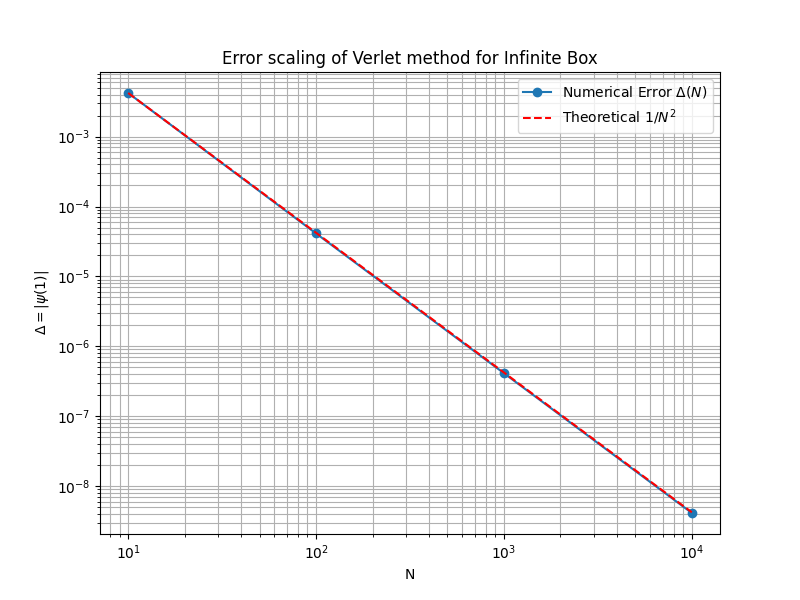
\includegraphics[width=0.7\textwidth]{task1_error.png}
    \caption{Log-log plot of the error $\Delta$ as a function of the number of mesh points $N$. The slope $\approx -2$ verifies the second-order accuracy of the integrator.}
    \label{fig:task1}
\end{figure}

\section{Problem 2: Eigenstates of the Infinite Box}
Using the shooting method with a binary search algorithm, we determine the first four eigenvalues for the infinite box potential. The theoretical eigenvalues are given by $E_n = \frac{n^2 \pi^2}{2}$. The results are summarized in Table \ref{tab:task2}.

\begin{table}[H]
    \centering
    \caption{Eigenvalues for the Infinite Box Potential ($L=1$).}
    \begin{tabular}{|c|c|c|}
    \hline
    $n$ & Exact $E_n$ & Numerical $E_n$ \\ \hline
    1 & 4.9348 & 4.9348 \\
    2 & 19.7392 & 19.7392 \\
    3 & 44.4132 & 44.4132 \\
    4 & 78.9568 & 78.9568 \\ \hline
    \end{tabular}
    \label{tab:task2}
\end{table}

The corresponding eigenstates are plotted in Figure \ref{fig:task2}.

\begin{figure}[H]
    \centering
    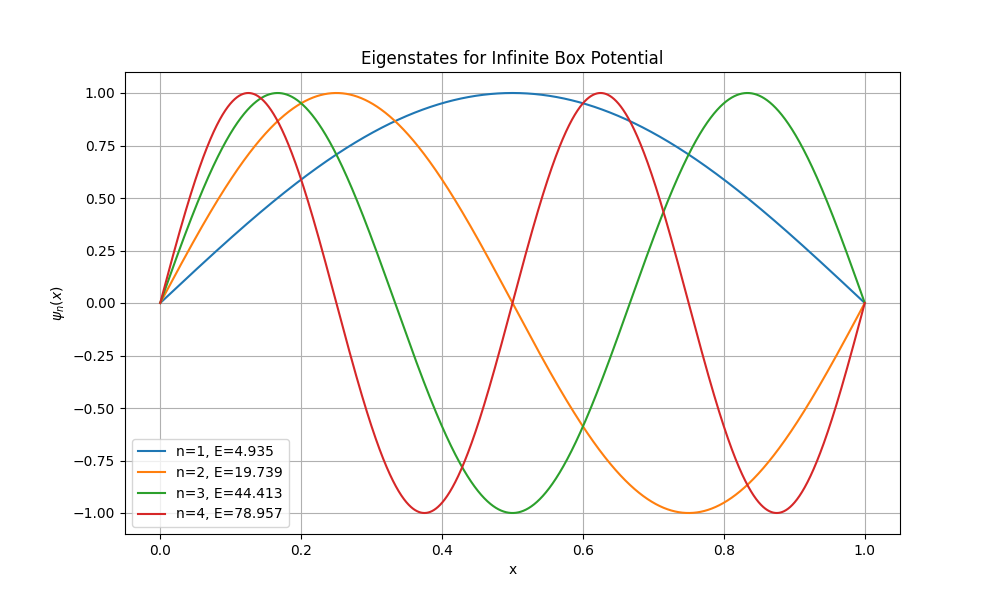
\includegraphics[width=0.7\textwidth]{task2_eigenstates.png}
    \caption{First four eigenstates of the infinite box potential.}
    \label{fig:task2}
\end{figure}

\section{Problem 3: Harmonic Oscillator}
We solve the TISE for the harmonic oscillator potential $V(x) = x^2/2$. Exploiting the symmetry of the potential, we integrate from $x=0$ to $x_{max}=5$. The boundary conditions at $x=0$ are $\psi(0)=1, \psi'(0)=0$ for even states and $\psi(0)=0, \psi'(0)=1$ for odd states. The exact eigenvalues are $E_n = n + 1/2$. The numerical results match the theoretical values perfectly as shown in Table \ref{tab:task3}.

\begin{table}[H]
    \centering
    \caption{Eigenvalues for the Harmonic Oscillator potential.}
    \begin{tabular}{|c|c|c|}
    \hline
    $n$ & Exact $E_n$ & Numerical $E_n$ \\ \hline
    0 & 0.5 & 0.5000 \\
    1 & 1.5 & 1.5000 \\
    2 & 2.5 & 2.5000 \\
    3 & 3.5 & 3.5000 \\ \hline
    \end{tabular}
    \label{tab:task3}
\end{table}

\begin{figure}[H]
    \centering
    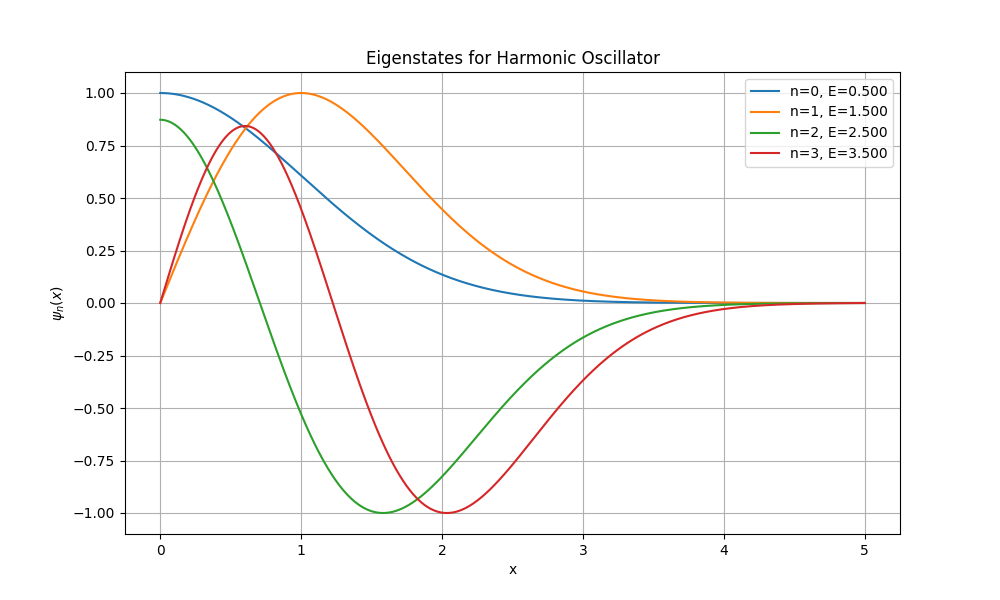
\includegraphics[width=0.7\textwidth]{task3_eigenstates.png}
    \caption{First four eigenstates of the harmonic oscillator.}
    \label{fig:task3}
\end{figure}

\section{Problem 4: Anharmonic Potential}
Finally, we consider the anharmonic potential $V(x) = \frac{1}{2}x^2 + \frac{1}{2}x^4$. This potential does not have a simple analytical solution. Using the same shooting method and parity conditions as in Problem 3, we find the first four eigenvalues.

\begin{table}[H]
    \centering
    \caption{Numerical Eigenvalues for the Anharmonic Potential $V(x) = x^2/2 + x^4/2$.}
    \begin{tabular}{|c|c|c|}
    \hline
    $n$ & Numerical $E_n$ & Parity \\ \hline
    0 & 0.6962 & Even \\
    1 & 2.3244 & Odd \\
    2 & 4.3275 & Even \\
    3 & 6.5784 & Odd \\ \hline
    \end{tabular}
    \label{tab:task4}
\end{table}

The eigenstates are shown in Figure \ref{fig:task4}. Note that these values are significantly higher than the harmonic oscillator values due to the additional $x^4$ term making the potential well steeper.

\begin{figure}[H]
    \centering
    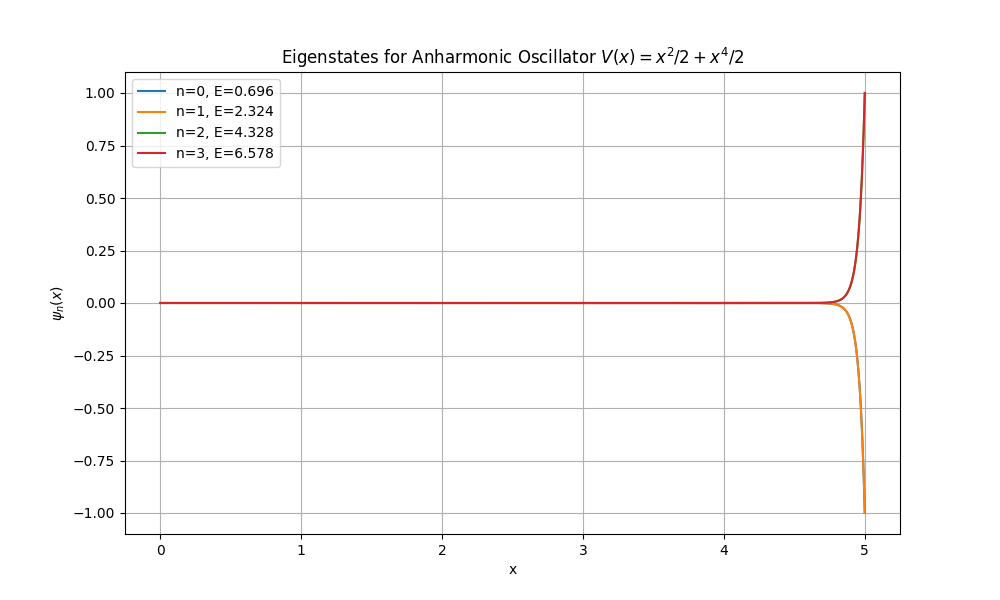
\includegraphics[width=0.7\textwidth]{task4_eigenstates.png}
    \caption{First four eigenstates of the anharmonic potential.}
    \label{fig:task4}
\end{figure}

\section{Conclusion}
The shooting method combined with a second-order integrator like the Velocity Verlet scheme is a powerful tool for finding eigenvalues and eigenstates of 1D quantum systems. We successfully verified the method on known cases (infinite box and harmonic oscillator) and applied it to an anharmonic potential where analytical solutions are unavailable.

\end{document}
